\documentclass[11pt]{article}
\usepackage{mystyle}

\title{Spherical Harmonic Update}
\author{Scott Trinkle}
\date{May 16, 2018}

\begin{document}

\maketitle



\section{From orientation data to SH}
The following is adapted from \cite{Alimi2018}:\newline

The spherical harmonics (SH) are defined as
\begin{align}
  Y_l^m(\theta, \phi) = N_l^m P_l^m(\text{cos}\theta)e^{jm\phi},
\end{align}
and form an orthonormal basis over $L_2(\mathbb{S}^2)$. Any
square integrable function $f(\theta, \phi) \in L_2(\mathbb{S}^2)$ can
be expressed as a linear combination of SH:
\begin{align}
  f(\theta, \phi) = \sum_{l=0}^{\infty}\sum_{m=-l}^l c_{lm}Y_l^m(\theta, \phi),
  \label{eq:SHexpand}
\end{align}
with coefficients $c_{lm}$ given by
\begin{align}
  c_{lm} = \int_{\mathbb{S}^2} f(\bm{w}) \bar{Y}_l^m(\bm{w}) \mathrm{d}\bm{w},
  \label{eq:coeffs_0}
\end{align}
where the overbar denotes conjugation and
\begin{align}
  \bm{w}(\theta, \phi) = [\text{sin}\theta\text{cos}\phi\text{, }  \text{sin}\theta \text{sin}\phi\text{, }  \text{cos}\theta]^T.
\end{align}

We are interested in determining the orientation distribution function (ODF)
$f(\theta, \phi)$ from the voxel-wise principal orientation vectors determined
from structure tensor analysis. In order to expand this function on
the SH, we model each orientation vector as a 2D Dirac delta function
$\delta$ on the sphere. That is, in a ROI containing $K$ voxels, our ODF
can be written as
\begin{align}
  f(\theta, \phi) = \frac{1}{K}\sum_{k=1}^K \delta(\theta - \theta_k)\delta(\phi - \phi_k).
\end{align}

If we substitute this into Eqn \ref{eq:coeffs_0}, then the sifting property of the Dirac
delta function can be used, and the integral reduces to:
\begin{align}
  c_{lm} = \frac{1}{K}\sum_{k=1}^K \bar{Y}_l^m(\theta_k, \phi_k).
\end{align}
A SH approximation $\hat{f}(\theta, \phi)$ can then be determined to an arbitrary
band-limit $L_{max}$ using Eqn \ref{eq:SHexpand}.

\section{Simplifications in HARDI literature}

Spherical harmonics are used extensively in the HARDI literature
to represents ODFs \cite{Tournier2004}. Generally, the following simplifications are made

\begin{itemize}
\item Diffusion is symmetric about the origin, so odd-ordered SH components are assumed zero and ignored
\item The diffusion-weighted signal and ODF are both real functions, so their SH representations exhibit conjugate symmetry
\end{itemize}

Accordingly, in the Dipy python package \cite{Garyfallidis2014}, only even-ordered spherical harmonic
components are calculated for the various HARDI reconstruction methods, and the
conjugate symmetry is exploited as follows:
\begin{align}
  Y_{l}^m(\theta, \phi)_{real} \equiv
  \begin{cases}
    \sqrt{2}\text{Re}\left[Y_l^{|m|}(\theta, \phi)\right] & m < 0\\
    Y_l^0(\theta, \phi) & m = 0\\
    \sqrt{2}\text{Im}\left[Y_l^m(\theta, \phi)\right] & m > 0\\
  \end{cases}
  \label{eq:real_Y}
\end{align}

\section{Applications to xray ODFs}

Figure \ref{fig:odfs} shows ODFs calculated with this method for both real xray data
and a simulated phantom with three groups of orthogonal fibers, using both even-only and
all SH components up to $L_{max} = 8$. The figures also lightly display the peak
estimate as a thin red line. These ODFs were generated using
$\sigma_d = 3 \text{ } \mu m$ and $\sigma_N = 6 \text{ } \mu m$ for the structure tensors. These
values were shown to have the highest AUC value in classifying fibers using the
fractional anisotropy metric. Further work will use the accuracy of the peak direction
estimate to tune these and other parameters.

We see that overall, the two ODFs identify similar peaks for both the even
and full SH representations. The symmetry is obviously lost when the odd
components are used, however. This is most obvious in the XYZ phantom.
In Figure \ref{fig:xyz_all}, we see that the structure tensor analysis
resulted in few orientations in the -z and +x directions, while that symmetry
is enforced with the even SH representation in \ref{fig:xyz_even}. For the
real data, the overall ODF shapes are more similar, but the peak estimate
is different.

\begin{figure}[h]
  \centering
  \begin{subfigure}[b]{0.3\textwidth}
    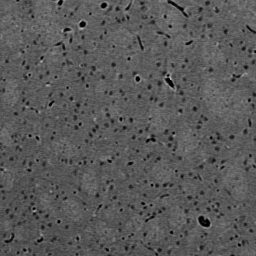
\includegraphics[width=\linewidth]{figs/xray_sl84}
    \caption{Data}
  \end{subfigure}
  \hspace{1em}
  \begin{subfigure}[b]{0.3\textwidth}
    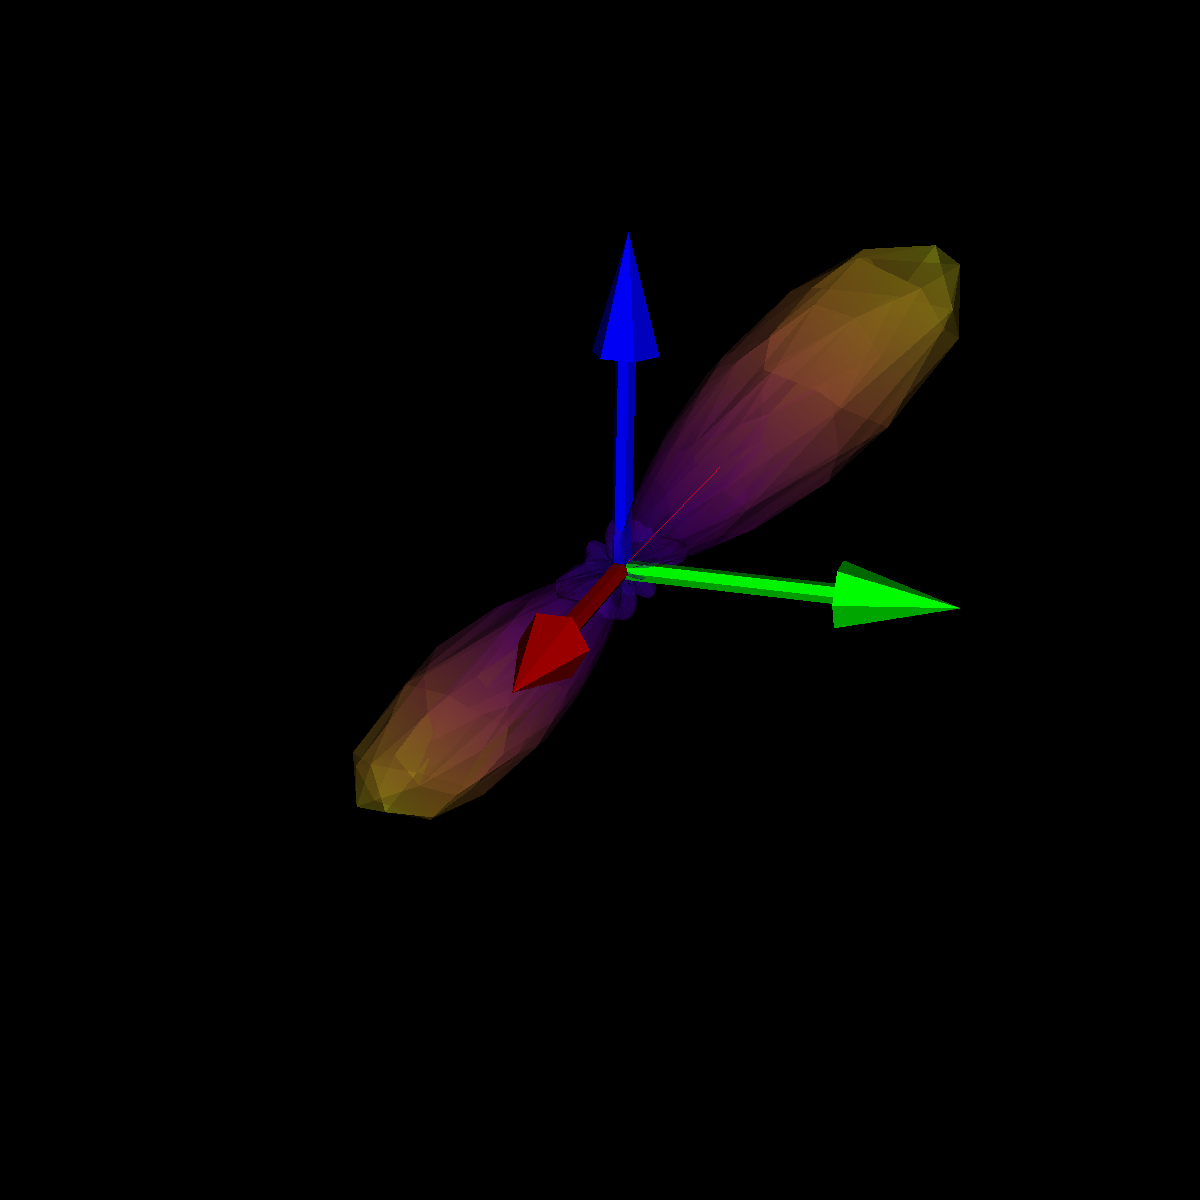
\includegraphics[width=\linewidth]{figs/roi_even}
    \caption{Data: even SH} 
  \end{subfigure}
  \hspace{1em}
  \begin{subfigure}[b]{0.3\textwidth}
    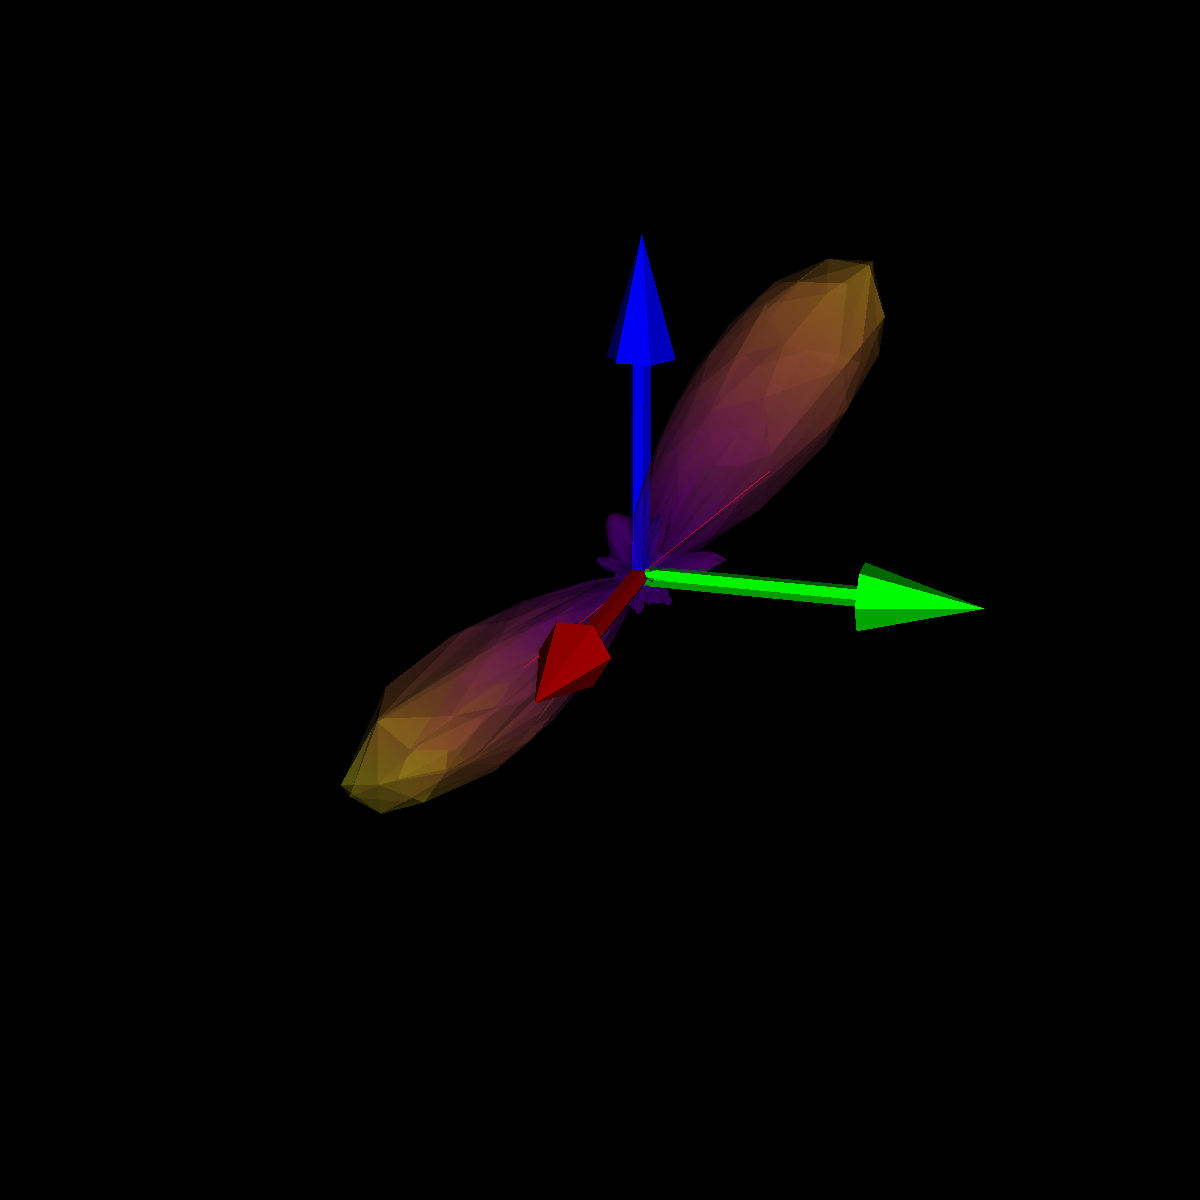
\includegraphics[width=\linewidth]{figs/roi_all}
    \caption{Data: all SH}
  \end{subfigure}
  \vspace{4em}
  \begin{subfigure}[b]{0.3\textwidth}
    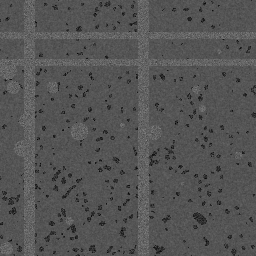
\includegraphics[width=\linewidth]{figs/xyz_phantom}
    \caption{XYZ Phantom}
  \end{subfigure}
  \hspace{1em}
  \begin{subfigure}[b]{0.3\textwidth}
    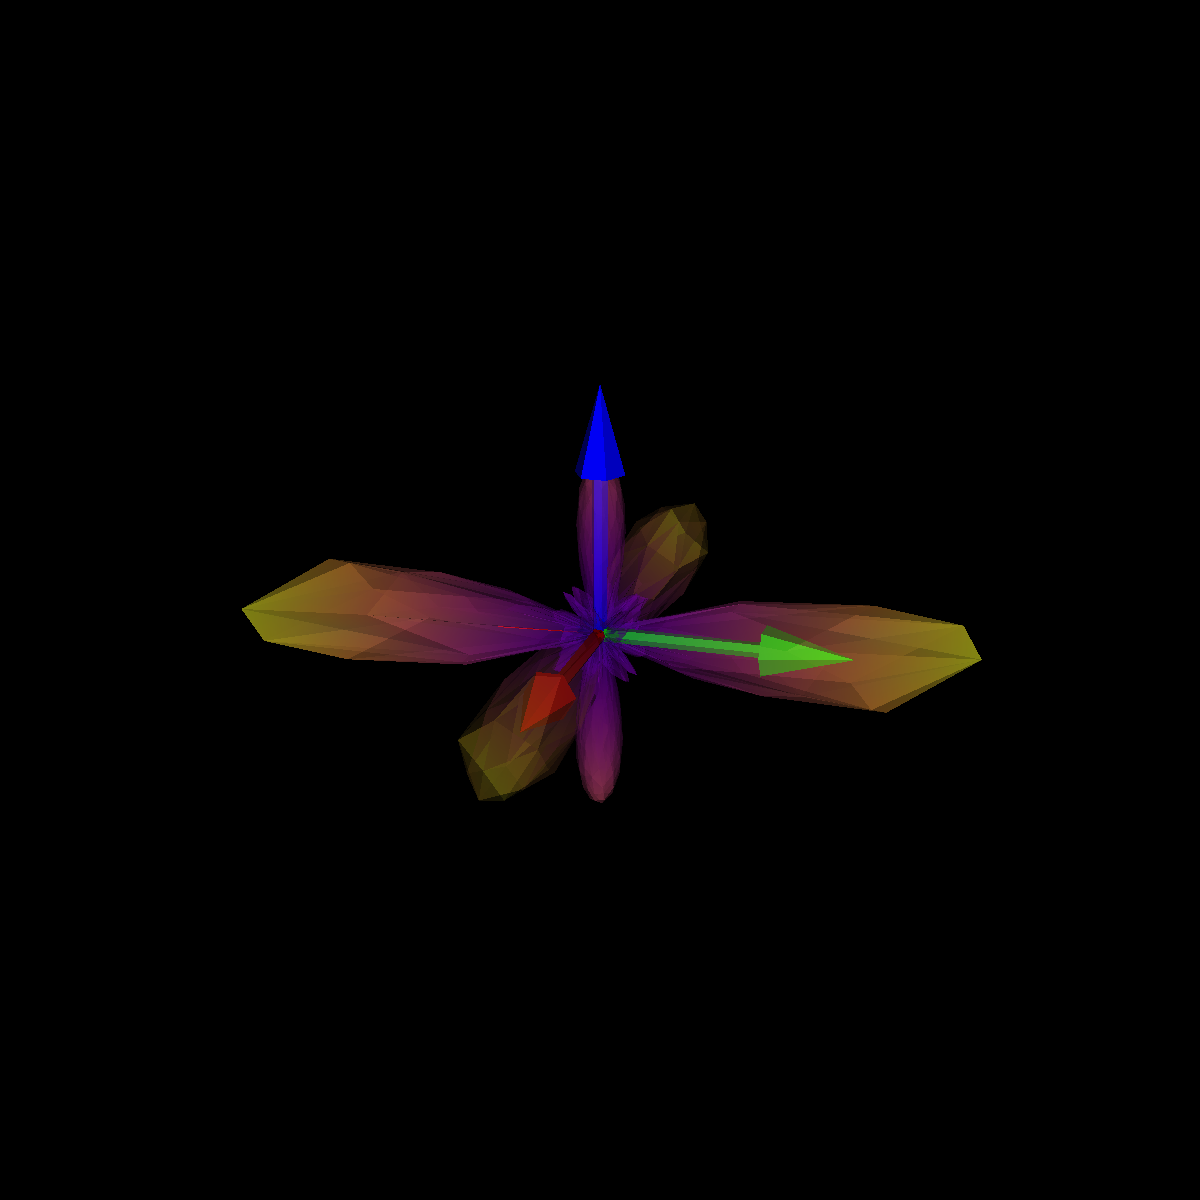
\includegraphics[width=\linewidth]{figs/phant_even}
    \caption{XYZ Phantom: even SH }
    \label{fig:xyz_even}
  \end{subfigure}
  \hspace{1em}
  \begin{subfigure}[b]{0.3\textwidth}
    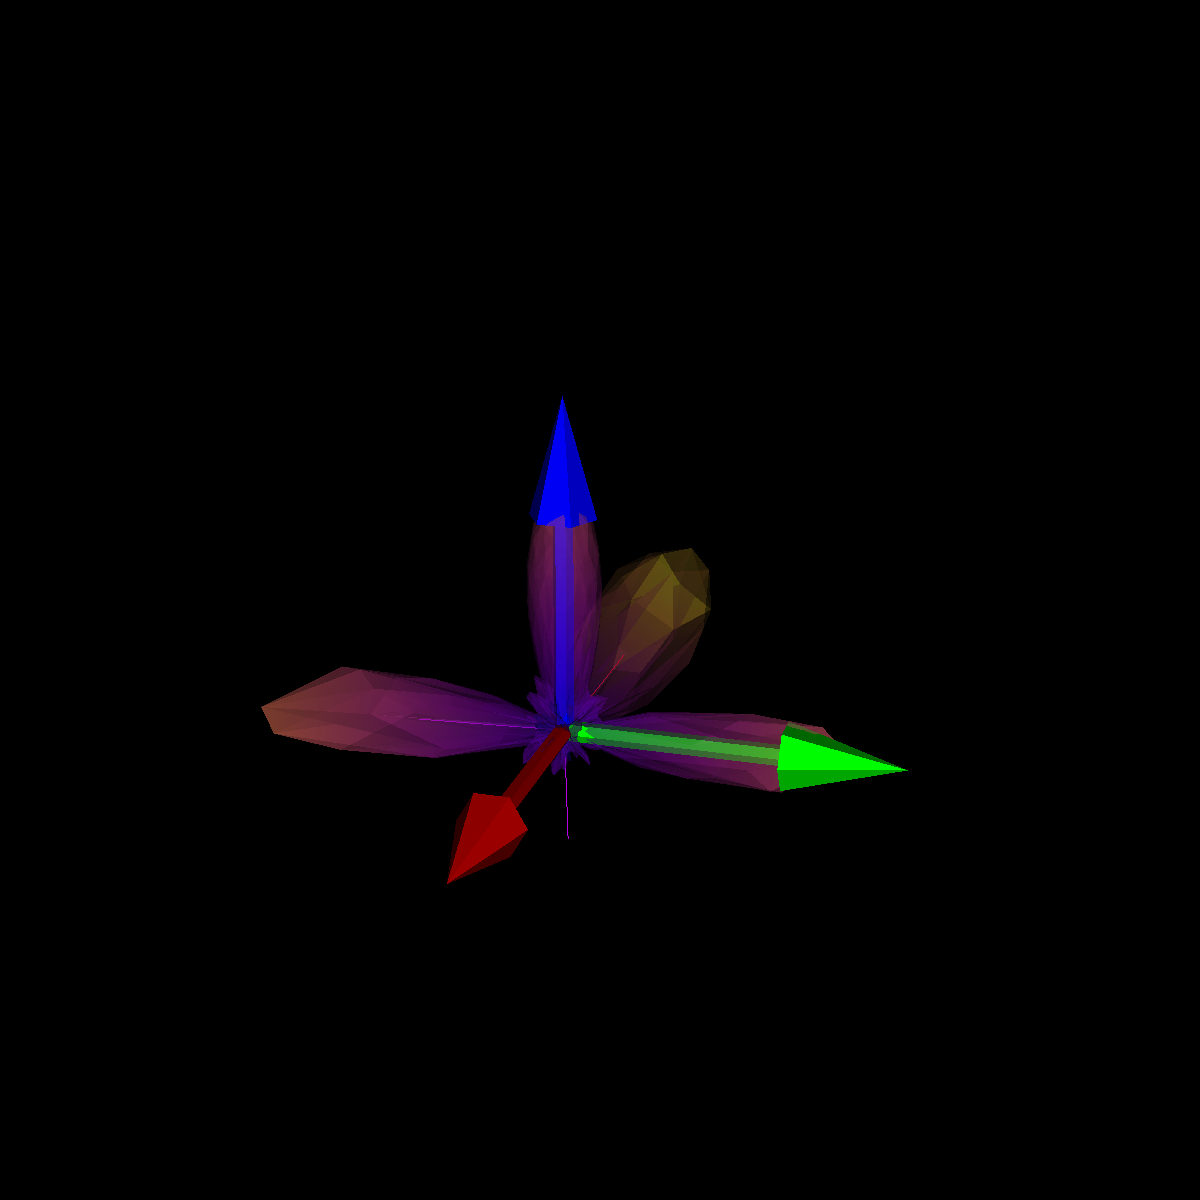
\includegraphics[width=\linewidth]{figs/phant_all}
    \caption{XYZ Phantom: all ODF}
    \label{fig:xyz_all}
  \end{subfigure}
  \caption{ODFs for $L_{max}$ = 8.}
  \label{fig:odfs}
\end{figure}

\bibliographystyle{ieeetr}
\bibliography{bib}
\end{document}
